Il est immédiat que l'on peut utiliser une repère orthonormé tel que l'on ait la situation suivante où la zone jaune indique les points non atteignables depuis la source $S$.


\begin{center}
	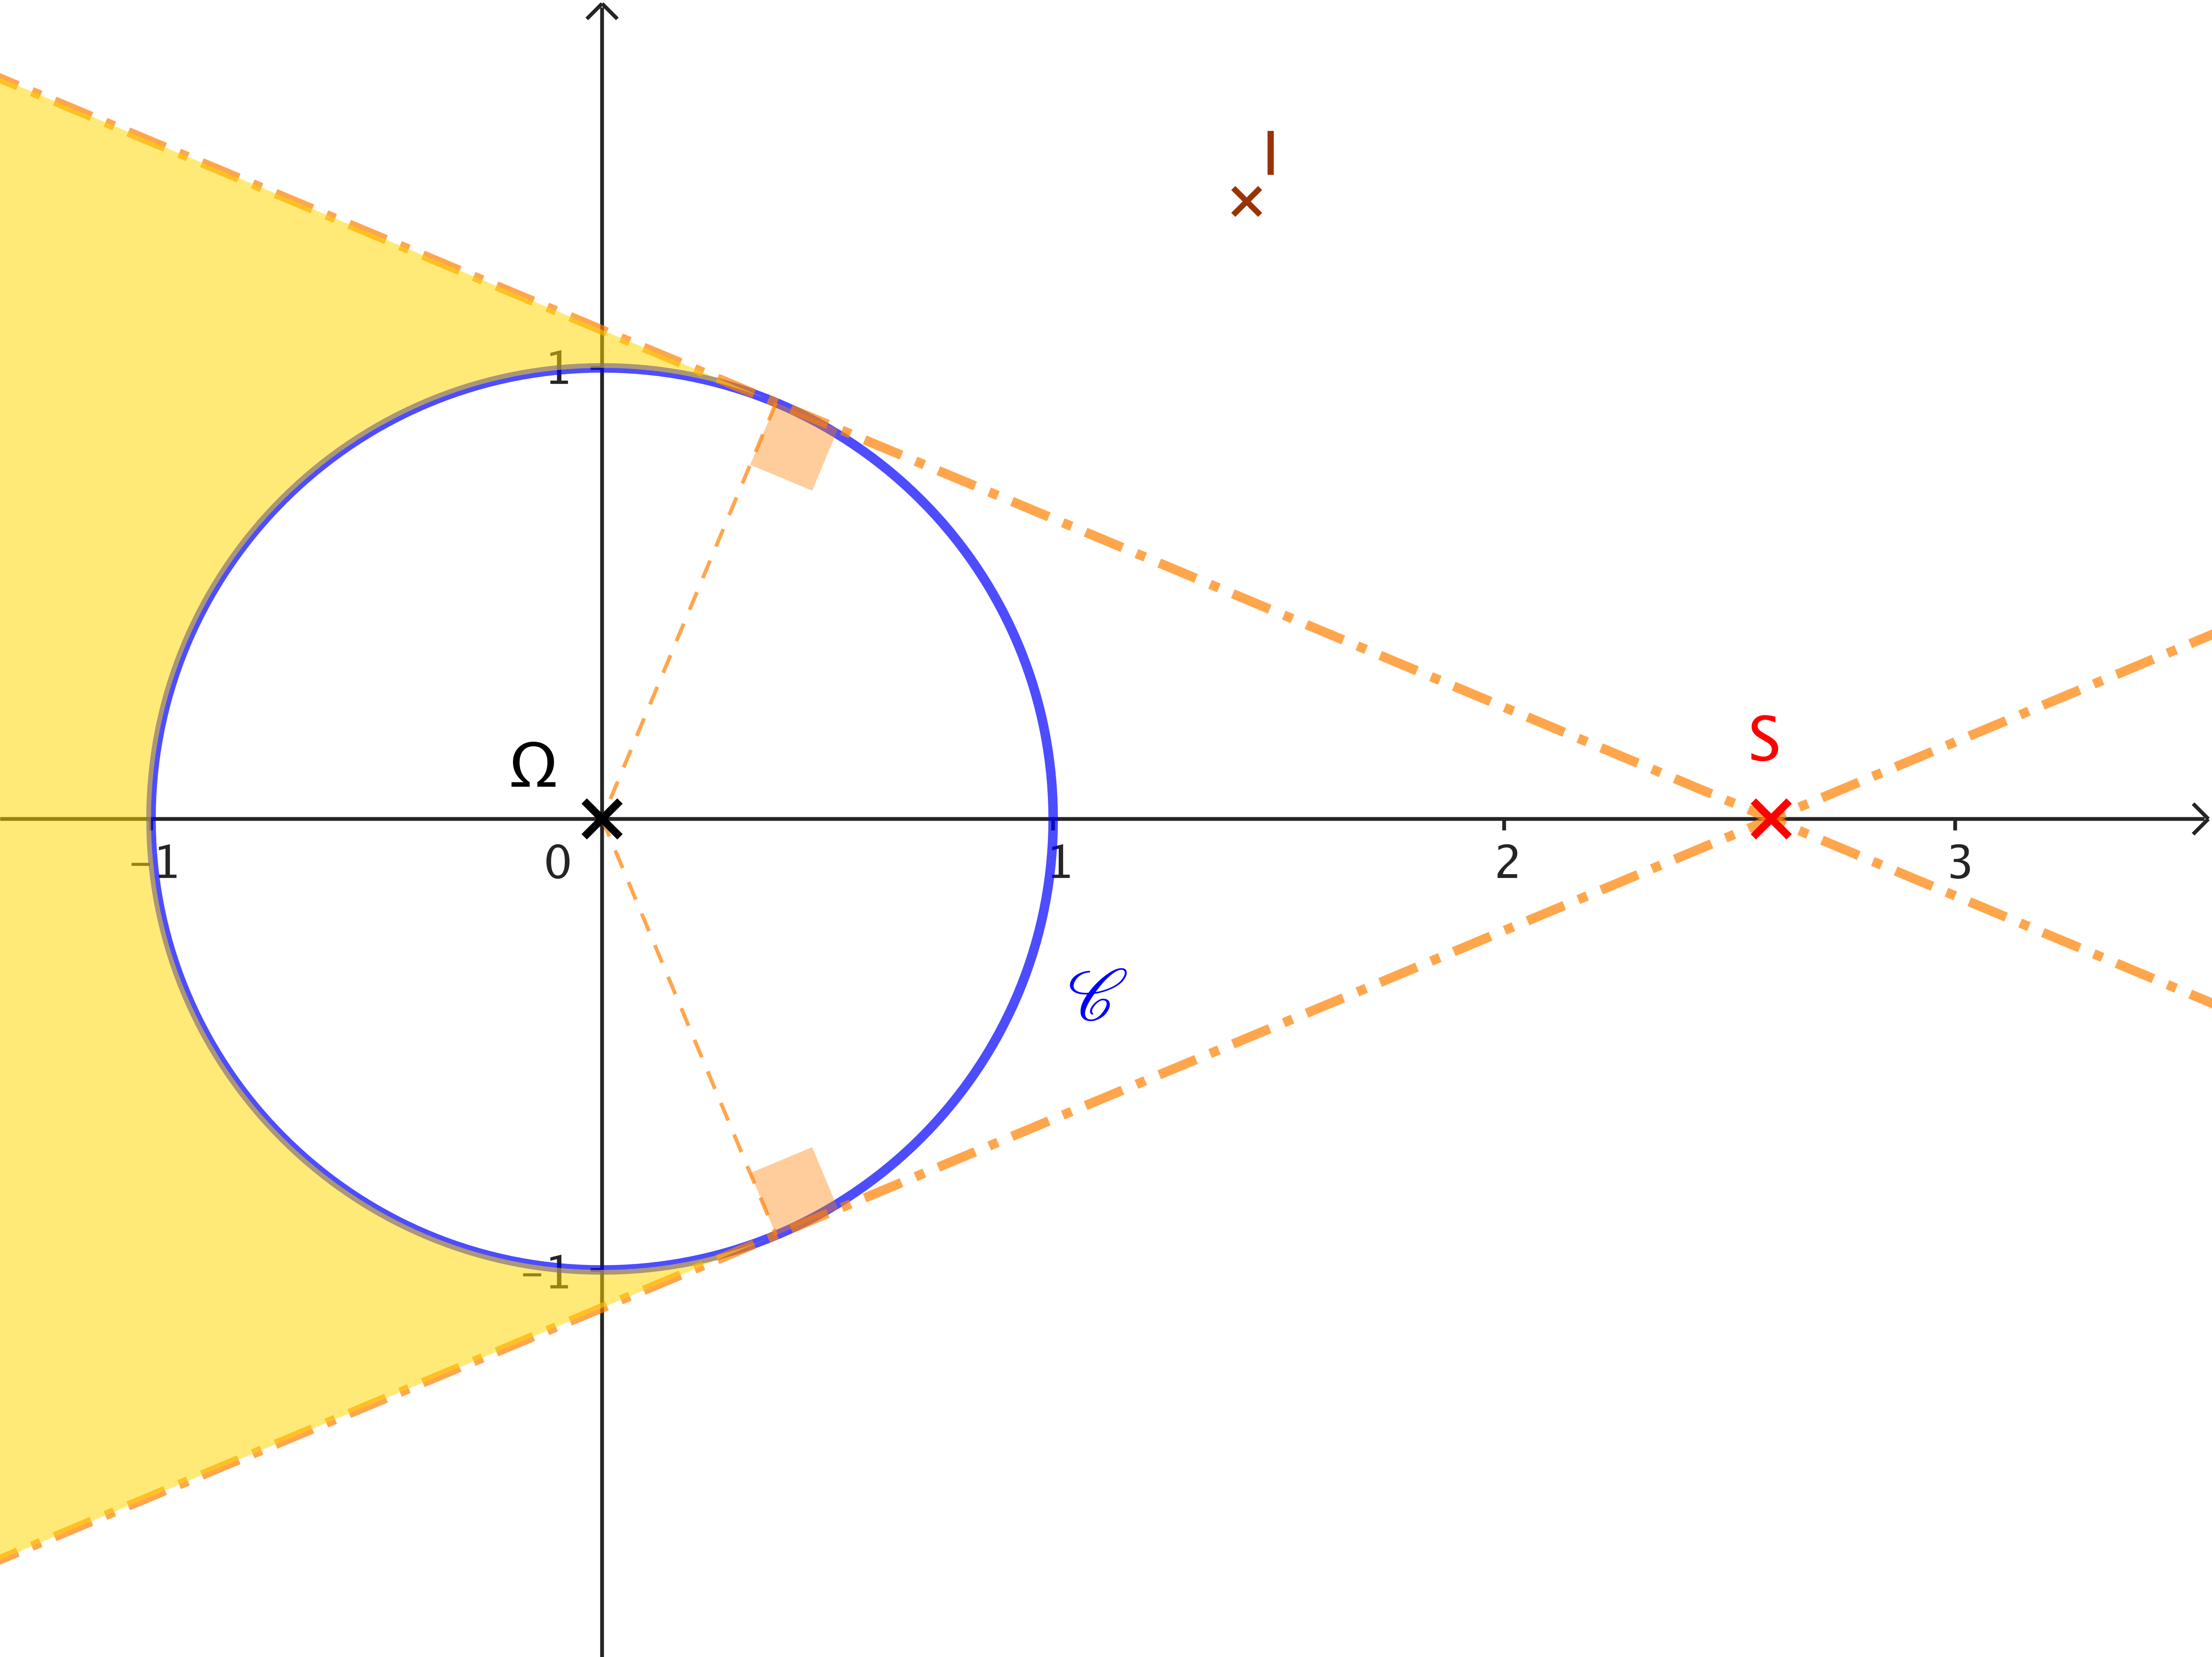
\includegraphics[scale=.75]{standard.png}
\end{center}


On utilise donc dans la suite les notations suivantes.

\begin{itemize}[label=\small\textbullet]
	\item $\setgeo{C} : x^2 + y^2 = 1$

	\item $S\coord{s | 0}$ avec $s > 1$

	\item $I\coord{i | j}$ est sur un rayon issu de $S$ après réflexion sur le miroir sphérique.

	\item $R\coord{x_R | y_R}$ est le point de contact recherché. Avec les choix faits ci-dessus, il est immédiat que $x_R > 0$ d'où $x_R = \sqrt{1 - y_R^2}$. Notre inconnue sera donc $y_R$ et non $x_R$. Notons que $y_R \in \intervalO{-1}{1}$.
\end{itemize}

